\documentclass[a4paper,12pt]{article} % тип документа

% report, book

% объявляем новую команду для переноса строки внутри ячейки таблицы
\newcommand{\specialcell}[2][c]{%
  \begin{tabular}[#1]{@{}c@{}}#2\end{tabular}}

%  Русский язык
\usepackage{multirow}
\usepackage{wrapfig}
\usepackage[T2A]{fontenc}			% кодировка
\usepackage[utf8]{inputenc}			% кодировка исходного текста
\usepackage[english,russian]{babel}	% локализация и переносы

\usepackage{indentfirst} %Красная строка
\usepackage[a4paper,top=1.3cm,bottom=2cm,left=1.5cm,right=1.5cm,marginparwidth=0.75cm]{geometry}
\usepackage[usenames]{color}
\usepackage{colortbl}

% Заметки
\usepackage{todonotes}

% Математика
\usepackage{amsmath,amsfonts,amssymb,amsthm,mathtools}
\usepackage{hyperref}


% Вроде для вставки кода
\usepackage{listings}
\usepackage{minted}
\usepackage{xcolor}


\begin{document}
\pagestyle{empty}
\begin{titlepage}
\begin{center}
    {\large МОСКОВСКИЙ ФИЗИКО-ТЕХНИЧЕСКИЙ ИНСТИТУТ (НАЦИОНАЛЬНЫЙ ИССЛЕДОВАТЕЛЬСКИЙ УНИВЕРСИТЕТ)}
\end{center}
\begin{center}
    {\largeФизтех-школа прикладной математики и информатики}
\end{center}


    \vspace{3.5cm}

\begin{center}
    
\includegraphics[width=0.4\linewidth]{hv_full.png}
\end{center}
\vspace{0.1cm}
{\huge
\begin{center}
    {\bf Подсчет числа $\pi$ с помощью \\ упругих соударений двух брусков}
\end{center}
}
\vspace{2cm}
\begin{flushright}
{\LARGE Автор:\\ Шалыгин Игорь Владимирович \\
\vspace{0.2cm}
Группа Б05 - 207}
\end{flushright}
\vspace{3.5cm}
\begin{center}
    Долгопрудный 2023
\end{center}
\end{titlepage}
\newpage
\pagestyle{plain}


\section*{Введение}
Представим себе идеальную модель, где происходят абсолютно упругие столкновения, где нет трения, и существуют два блока масс $m_1$, $m_2$. Также в этой системе есть стена.

В такой системе будет можно будет наблюдать следующее явления: если запустить с некоторой скоростью брусок с массой $m_1$, где $m_1 = m_2 \cdot 100^n, n \in \mathcal{N}_0$, в направлении тела с массой $m_2$, которое будет расположено строго между стеной и первым телом, то суммарное количество соударений бруска массой $m_2$ со стеной и с первым бруском будет равно числу, состоящему из первых $n + 1$ цифр числа $\pi$.


\section*{Теория}
Для начала разберемся, что происходит после столкновения блоков. Так как соударения абсолютно упругие, то в лабораторной системе отсчета выполняются законы сохранения импульса и энергии \newline ($v_1' < 0$ - начальная скорость первого бруска):

\[
\begin{matrix}
    \left\{
    \begin{matrix}
        \frac{m_1 \cdot v_1^2}{2} + \frac{m_2 \cdot v_2^2}{2} = \frac{m_1 \cdot (v_1')^2}{2} &
        \mbox{(ЗСЭ)} \\
        m_1 \cdot v_1 + m_2 \cdot v_2 = m_1 \cdot v_1' &
        \mbox{(ЗСИ)}
    \end{matrix}
    & \Rightarrow &
    \left\{
    \begin{matrix}
        \left(\frac{v_1}{\sqrt{m_2}}\right)^2 + \left(\frac{v_2}{\sqrt{m_1}}\right)^2 = const &
        \mbox{(*)}
        \\
        m_1 \cdot v_1 + m_2 \cdot v_2 = const &
        \mbox{(**)}
    \end{matrix}
\end{matrix}
\]

Возьмем координатные оси такие, что $y = \sqrt{m_2} \cdot v_2$, $x = \sqrt{m_1} \cdot v_1$. Тогда получим, что уравнение (*) - это уравнение окружности, а (**) - уравнение прямой с угловым коэффициентом $k = -\sqrt{\frac{m_1}{m_2}}$. После подстановки x и y получаем следующие уравнения:

\[
    \left\{
    \begin{matrix}
        x^2 + y^2 = m_1 \cdot (v_1')^2 &
        \mbox{(1)}\\
        \sqrt{m_1} \cdot x + \sqrt{m_2} \cdot y = const &
        \mbox{(2)}
    \end{matrix}
\]

Рассмотрим окружность (1). До первого соударения мы находимся в точке $A(v_1', 0)$. Далее после соударения новую точку получаем из пересечения оружности и прямой, проходящей через точку $A$ с коэффициентом $k = -\sqrt{\frac{m_1}{m_2}}$. Следующим происходит соударение со стенкой, откуда мы получаем следующую точку, характеризующую движение элементов системы, $C$ из пересечения вертикальной прямой и окружности (упругое соударение со стеной меняет знак скорости бруска $m_2$ на противоположный). Таким образом, мы получили геометрический смысл данной задачи. Условие прекращения соударений - $0 \leq v_2 \leq v_1$, т.е. второй брусок не движется к стенке (в ином случае произойдет как минимм одно соударение) и скорость второго бруска меньше или равна скорости (в ином случае второй брусок догонит первый). Таким образом, получаем дугу окружности, где столкновения останавливаются.

\bigskip

\begin{minipage}{0.5\textwidth}
Например, для $0.087$ радиан (10$^\circ$) график будет выглядеть так. 
\begin{enumerate}
    \item Начальное положение системы - точка B
    \item Конечное положение - точка D'
    \item Зона прекращения соударений - малая дуга DD'. Точки D и D' включительно, что следует из нестрогого неравенства. На рисунке выделена красным цветом.
    \item Пунктрирные векторы обозначают, как изменялось состояние системы с течением времени.
\end{enumerate}
\end{minipage}
\begin{minipage}{0.55\textwidth}
\begin{center}
    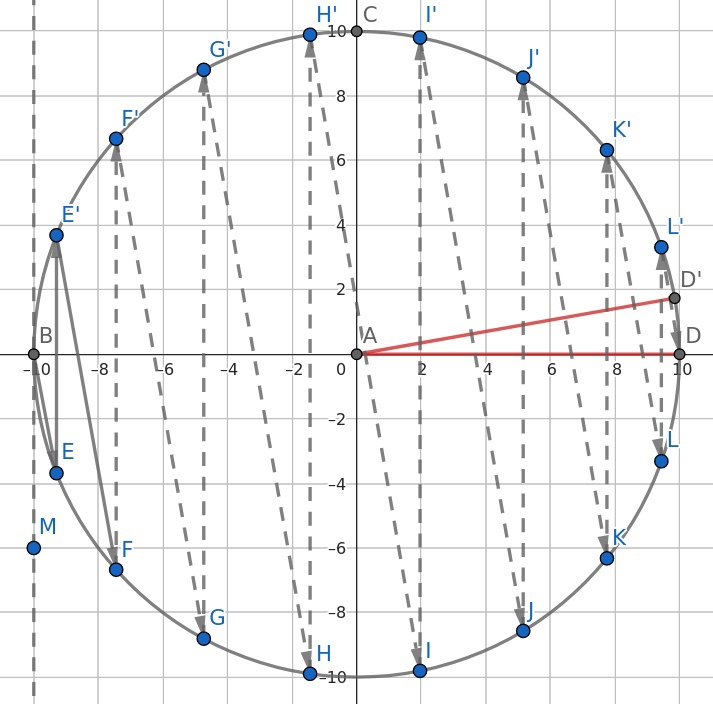
\includegraphics[width=0.65\linewidth]{CircleExample.jpg}
\end{center}
\end{minipage}

\newpage

Следующим шагом заметим один важный факт. Каждый раз при соударении мы "отрезаем" от изначальной окружности дугу длиной $2 \varpi \cdot v_1'$ (длина дуги напрямую следует из теоремы о вписанном угле), где $\varphi = arctg(-\frac{1}{k}) = arctg(\sqrt{\frac{m_2}{m_1}})$. На рисунке выше $\angle BEE' = \dots = \angle K'LL' = \angle LL'D = \varphi = \angle MBE$ (из соображений геометрии).

Таким образом, получаем, что количество соударений - это максимальное $n \in \mathcal{N}_0$ такое, что
\[n \cdot (2 \cdot \varphi) \leq (2 \cdot \pi)\]
\[ n \cdot \varphi \leq \pi\]

Рассмотрим значения $\varphi$:

\begin{center}
\begin{tabular}{|c|c|c|c|}
\hline
 Отношение масс & $\varphi$ формула & $\varphi$ значение & $n_{max} \in \mathcal{N}$\\ \hline
 $m_1 : m_2$ & $arctg(\sqrt{\frac{m_2}{m_1}})$ & & $n_{max} \cdot \varphi \leq \pi < (n_{max} + 1) \cdot \varphi$\\ \hline
 $10^0 : 1$ & $arctg(\frac{1}{1})$ & $0.7853981\dots$ & 3
 \\ \hline
 $10^2 : 1$ & $arctg(\frac{1}{10})$ & $0,0996686\dots$ & 31 \\ \hline
 $10^4 : 1$ &  $arctg(\frac{1}{10^2})$ & $0,0099996\dots$ & 314\\ \hline
 $10^6 : 1$ &  $arctg(\frac{1}{10^3})$ & $0,0009999\dots$ & 3141\\ \hline
 $10^8 : 1$ &  $arctg(\frac{1}{10^4})$ & $0,0000999\dots$ & 31415\\ \hline
 $10^{10} : 1$ &  $arctg(\frac{1}{10^5})$ & $0,0000099\dots$ & 314159\\ \hline
\end{tabular}
\end{center}

Мы знаем, что при стремлении $x$ к 0, $arctg(x) \approx x$, то есть получим, что количество столкновений будет равно $[\pi \cdot 10^n]$ (<<[ ]>> обозначают целую часть выражения).

Подставляя полученные значения $\varphi$ для отношений масс из таблицы получаем верные соотношения. С увеличением отношения масс мы увеличиваем точность $\varphi$, и из разложения $tg(\varphi)$ по Тейлору в нуле, мы можем заметить, что и погрешность линейно зависит от $\varphi^3$, т.е. с уменьшением $\varphi$ убывает и притом с большей скоростью, чем линейная.


\section*{Практика. Создание модели на компьютере}
Из-за невозможности провести эксперимент вживую я решил его запрограммировать. Для этого было создано полноценное приложение с помощью библиотеки pygame с анимированными брусками и возможностью задание параметров брусков.

Для работы с брусками я создал класс Block. Ниже указаны его методы

\begin{minted}{Python}

class Block:

    def print_on_screen(self, screen, color: tuple):
        '''
        :param screen: Экран pygame
        :param color: Цвет выводимого прямоугольника
        :return: pygame.draw.rect(), рисующую прямоугольник в нужной позиции
        '''

    def update_position(self) -> None:
        '''
        Прибавляет к координате скорость за единицу времени
        '''



    @staticmethod
    def collide(l_block, r_block) -> bool:
        '''
        :param l_block: Левый объект Block
        :param r_block: Правый объект Block
        :return: Выполнены условия столновения (один зашел за границы второго)
        '''

    @staticmethod
    def bounce(l_block, r_block) -> None:
        '''
        Устанавливает объектам новые скорости после столкновения
        Используются формулы, выведенные из ЗСИ и ЗСЭ
        :param l_block: Левый объект Block
        :param r_block: Правый объект Block
        '''
        
    def wall_collide(self) -> bool:
        '''
        :return: Выполнено ли условие выхода за левый край экрана (стену)
        '''
        
    def reverse_vel(self) -> None:
        '''
        Изменяет скорость на противоположную
        '''
\end{minted}

Для подсчета скоростей блоков после упругого столкновения в методе $collide$ используем формулы, выведенные из ЗСИ и ЗСЭ ($v_1$ и $v_2$ - скорости после столкновения, $v_1'$ и $v_2'$ - до столкновения):

\[
\begin{matrix}
    v_1 = \frac{2m_2v_2' + v_1'(m_1-m_2)}{m_1+m_2}
    \\
    v_2 = \frac{2m_1v_1' + v_2'(m_2-m_1)}{m_1+m_2}
\end{matrix}
\]

Программа подсчитывает количество ударов за счет моделирования каждого столкновения по отдельности, вследствие чего при больших $n$ работает продолжительное время, но демонстрирует достоверность полученных результатов.

\begin{center}
    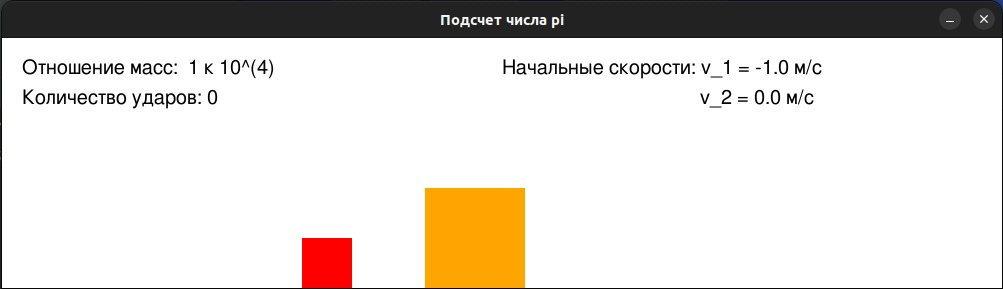
\includegraphics[width=0.7\linewidth]{ProgPic.jpg}
\end{center}

\newpage


\section*{Явление в релятивизме}
Следующим шагом я решил проверить, будет ли существовать данное явление в релятивистской механике. Согласно гипотезе, данное явление должно выполняться, иначе мы сможем отличить одну инерциальную систему отсчета от другой.

Для проверки изменим программу, чтобы она считала соударения по релятивистским формулам. Для определения результатов соударения будем:
\begin{enumerate}
    \item Переходить из ЛСО в инерционную СО
    \item Изменять импульсы тел на противоположные вследствие упругого соударения
    \item Переходить из инерционной СО обратно в ЛСО
\end{enumerate}

\bigskip

Найдем $\beta = \frac{V}{c}$, где $V$ - скорость инерционной системы отсчета для двух блоков: 

\[
m_1\frac{\beta_1 + \beta}{1 + \beta_1 \cdot \beta} + m_2\frac{\beta_2 + \beta}{1 + \beta_2 \cdot \beta} = 0 \ \Rightarrow
\]

\[
\beta^2(m_1\beta_2 + m_2\beta_1) + \beta(m_1 + m_2)(1 + \beta_1\beta_2) + (m_1\beta_1 + m_2\beta_2) = 0
\]

\[
\begin{matrix}
    \left\{
    \begin{matrix}
        a = m_1\beta_2 + m_2\beta_1 \\
        b = (m_1 + m_2)(1 + \beta_1\beta_2) \\
        c = m_1\beta_1 + m_2\beta_2 \\
        \beta = \dfrac{\sqrt{b^2 - 4ac} \pm b}{2a}
    \end{matrix}
\end{matrix}
\]

Выбираем минус, так как второе решение по модулю больше 1.

\[
\beta = \dfrac{\sqrt{b^2 - 4ac} - b}{2a}
\]

Таким образом, по закону сложения скоростей $\beta_1$ проходит следующие преобразования при упругом соударении с другим телом:

\[
\beta_1 \ \rightarrow \ \frac{\beta_1 + \beta}{1 + \beta_1 \cdot \beta} \ \rightarrow \ \beta_1' \ \text{:}= - \frac{\beta_1 + \beta}{1 + \beta_1 \cdot \beta} \ \rightarrow \ \frac{\beta_1' - \beta}{1 - \beta_1' \cdot \beta}
\]

\medskip

Для $\beta_2$ аналогично.

\section*{Заключение}
В ходе данной работы мне удалось исследовать такое явление, как получение числа $\pi$ с помощью упругого соударения двух блоков. Было дано геометрическое обоснование данного явления, теория подтерждена в релятивистской механике и построены модели на языке python, подтвердившие полученные результаты.

\end{document}
